The gather communication pattern gathers input data elements together from different places in memory and computes a single output result.
This is different from the map pattern since this pattern maps multiple inputs to a single output.
In this way the gather pattern has a many-to-one correspondence between inputs and outputs as can be seen in \autoref{fig:gather}.

\begin{figure}[ht]
	\centering
	\fbox{
		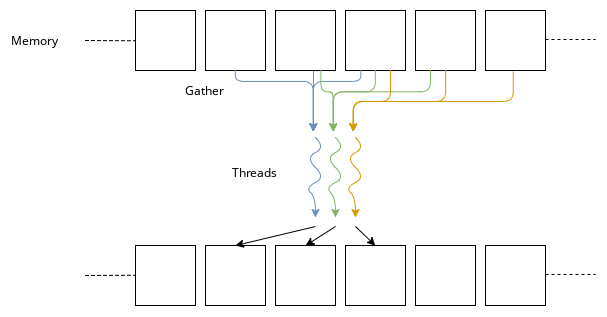
\includegraphics[width=0.6\textwidth]{figs/patterns/parallelgather.png}
	}
	\caption{Gather Pattern}
	\label{fig:gather}
\end{figure}

This parallel communication pattern can for instance be applied to image processing applications such as implementing blurring, sharpening, edge detection and more on an image.
This is done by 'sliding' a \textit{kernel} \footnote{Sometimes also called a \textit{convolutional matrix} or \textit{mask}} over the entire image to get a new image with a desired effect.
The effect which is applied to the new image is determined by the values in the kernel, but the parallel pattern which is used to implement this is the same, namely the gather pattern.
An example of applying a kernel to an image is seen in \autoref{fig:kernel}.
\begin{figure}[ht]
	\centering
	\fbox{
		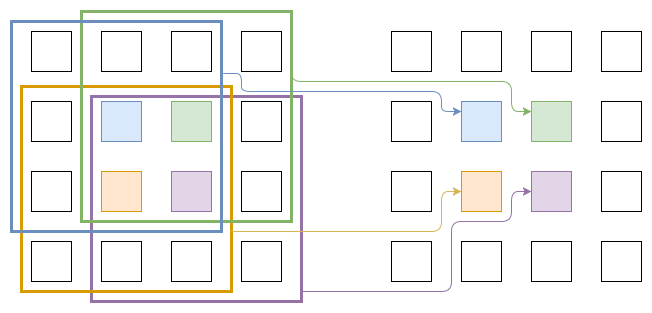
\includegraphics[width=0.6\textwidth]{figs/patterns/parallelblur2.png}
	}
	\caption{Example of a kernel operation with $\mathtt{4x4}$ dimensions}
	\label{fig:kernel}
\end{figure}
Using such a parallel communication pattern can vastly improve the computation time of applying for instance a kernel to an image.
Say that with a kernel with $\mathtt{NxN}$ dimensions and an image with $\mathtt{K}$ pixels the running time would be $\mathtt{O(N\cdot K)}$ on a serial processor compared to $\mathtt{O(N)}$ in parallel, assuming that $K$ threads can be spawned on the GPU.

%TODO: make small code example of gather